\documentclass[a4paper,12pt]{article}
\usepackage[utf8]{inputenc}
\usepackage[english]{babel}
\usepackage{graphicx}
\usepackage{ragged2e}
\usepackage{geometry}
\renewcommand{\baselinestretch}{1.2}
\usepackage{comment}
\usepackage{amssymb}
\usepackage{hyperref}
\usepackage{url}
\usepackage{listings}
\usepackage{color}
\usepackage{xcolor}

% for tikz package (flowchart)

\usepackage{tikz}
\usetikzlibrary{shapes.geometric, arrows}

\tikzstyle{startstop} = [rectangle, rounded corners, minimum width=3cm, minimum height=1cm,text centered, draw=black,]

\tikzstyle{io} = [trapezium, trapezium left angle=70, trapezium right angle=110, minimum width=3cm, minimum height=1cm, text centered, draw=black, ]

\tikzstyle{process} = [rectangle, minimum width=3cm, minimum height=1cm, text centered, draw=black, ]

\tikzstyle{decision} = [diamond, minimum width=3cm, minimum height=1cm, text centered, draw=black,]


\tikzstyle{arrow} = [thick,->,>=stealth]

%listings

\definecolor{mygreen}{HTML}{087012}
\definecolor{mygray}{HTML}{7e7f81}
\definecolor{mymauve}{HTML}{cb5be2}

\lstset{ 
  language=C,
  backgroundcolor=\color{white},  
  basicstyle=\footnotesize,        % size of fonts
  breaklines=true,                 % automatic line breaking
  captionpos=b,                   
  commentstyle=\color{mygreen},    % comment style
  keywordstyle=\color{blue},       % keyword style
  stringstyle=\color{mymauve},     % string literal style
}


\begin{document}
\begin{center}
\textbf{Assignment-8 \\
\bigskip
ELP - 718 Telecom Software Laboratory \\
\smallskip
Devendra Khatri \\
2018JTM2243 \\
2018-2020} \\
\vspace{10mm}
A report presented for the assignment on \\
Python \& GitHub\\
\vspace{30mm}

\includegraphics[scale=0.5]{logo} \\
\vspace{10mm}
Bharti School Of \\
Telecommunication Technology and Management \\
IIT Delhi \\
India \\
September 27, 2018
\end{center}
\newpage
\tableofcontents
\newpage
\listoffigures
\newpage

\section{Problem Statement 1}
\subsection{Problem Statement}
\cite{d1}
IIT Delhi, has just got the strongest computer. The professors in charge wants to check the computational capacity of the computer. So, they decided to create the problem which is to be given as an assignment to students. Can you help the professor to check the computation capability of the computer\\
A valid cross is defined here as the two regions (horizontal and vertical) of equal lengths crossing over each other. These lengths must be odd, and the middle cell of its horizontal region must cross the middle cell of its vertical region.
\vspace{1cm}
%\includegraphics[scale=.5]{}

%\includegraphics[scale=.5]{table.png}
\subsection{specification}
\begin{itemize}
	\item Detect the "S".
	\item If the number of S is cross equal and 4 direction. 
	\item find the odd number of square.
	\item Taking max1 and max2 number of squares.
	\
\end{itemize}
\subsection{Assumptions}
\begin{itemize}
\item Commond line argument input.
\item The 2-D matrix formation.
\end{itemize}

\newpage

\subsection{Program Structure}
\begin{figure}[h]
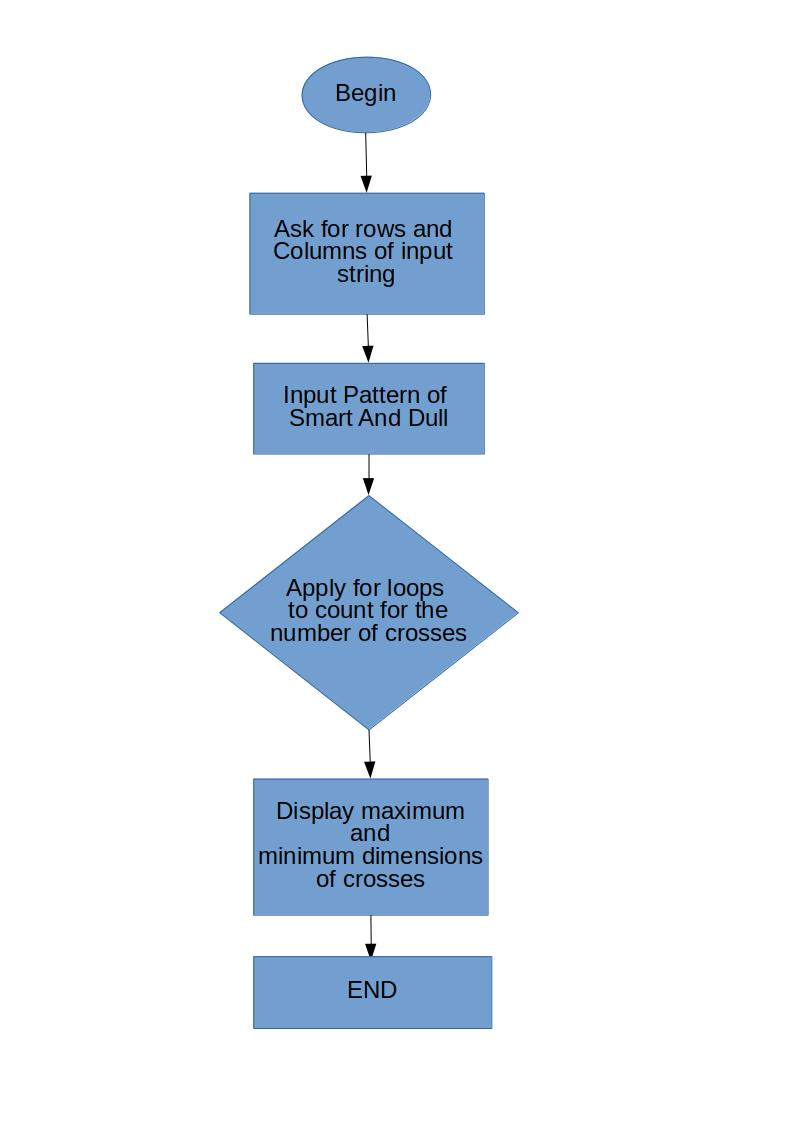
\includegraphics[scale=0.5]{ps1flow.jpg}
\caption{flowchart for ps1}
\label{fig:flow}
%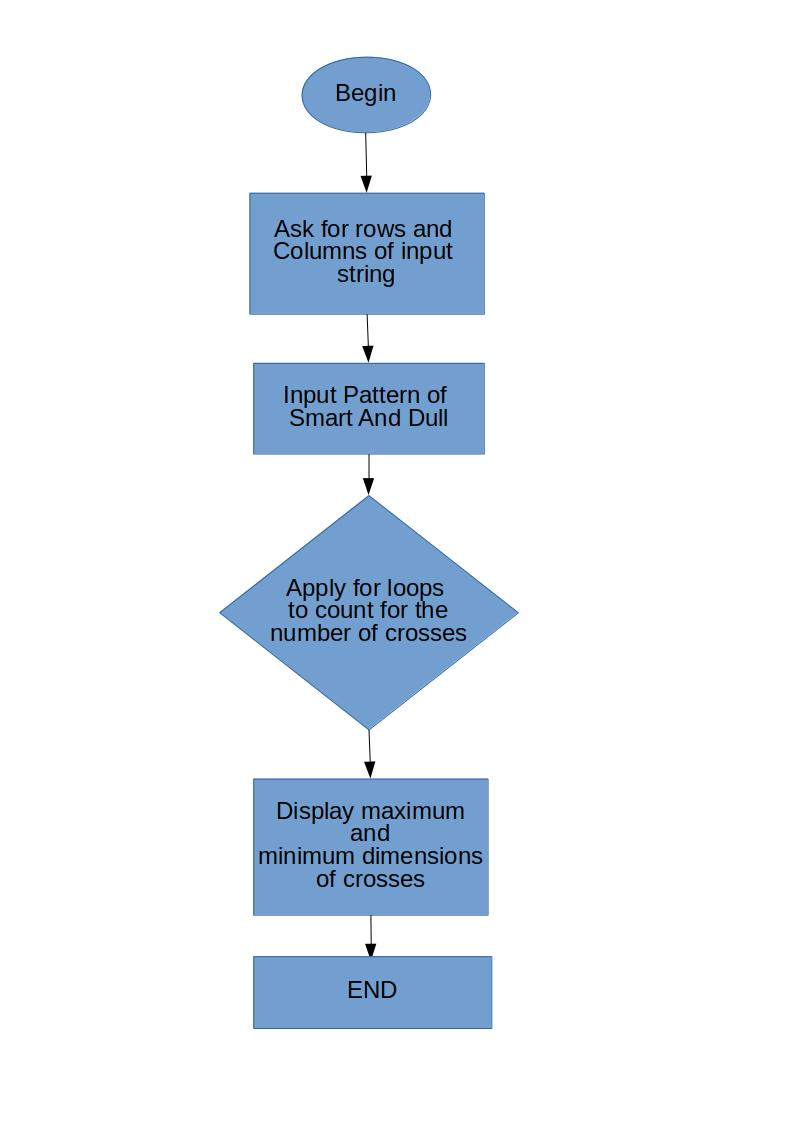
\includegraphics[scale=.5]{ps1flow.png}
\end{figure}

\subsection{Algorithm and Implementation}
\begin{itemize}
\item Store the elements in 2-D list
\item Using i,j parameter access each element.
\item When a "s" detected we find the near by "S" and cunt increased.
\item Select min value from them. and store in new list correspond the each.
\end{itemize}

\subsection{Input and Output format}
\begin{itemize}
    \item \textbf{Input Format}
    5 6\\
    SSSSSS\\
    SDDDSD\\
    SSSSSS\\
    SSDDSD\\
    SSSSSS
     \item \textbf{Output Format}. \\
     5 1 
     
      
\end{itemize}

\subsection{Test Cases}
\begin{enumerate}
    \item 6 6\\
    DSDDSD\\
    SSSSSS\\
    DSDDSD\\
    SSSSSS\\
    DSDDSD\\
    DSDDSD\\
    
    
\end{enumerate}
\begin{enumerate}
	\item 5 9\\
    SSSSDSDDD\\ 
	DDSDDDDDD\\
	SSSSSDDDD\\
	DDSDDSDDD\\
	DSSSDDDDD\\

	
	
\end{enumerate}

\subsection{Output}
\begin{enumerate}
    \item 9 1
\end{enumerate}



\subsection{Screen-shots}
\begin{figure}[h]
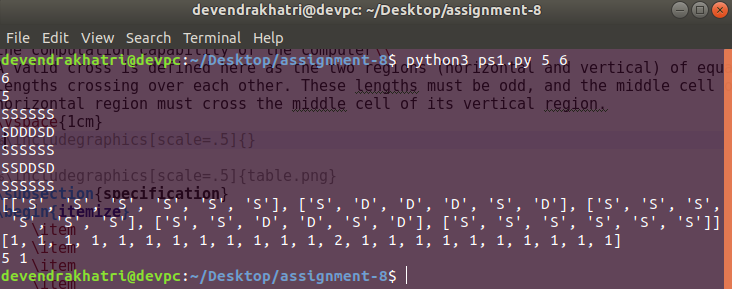
\includegraphics[scale=0.5]{PS1.png}
\caption{ps1- Decision 1}
\label{fig:ps1in}
\end{figure}





\newpage
\section{Problem Statement 2}
\subsection{Problem Statement}
\cite{problem2}
After, getting mix results of valid crosses, professors decided to test the computation abilities on one more problem. This time professors wanted to test the decryption capabilities of the computer.\\
Encryption of  a message requires three keys, k1, k2, and k3. The 26 letters of English and underscore are divided in three groups,  [a-i] form one group, [j-r] a second group, and everything else ([s-z] and underscore) the third group. Within each group the letters are rotated left by ki positions in the message. Each group is rotated independently of the other two. Decrypting the message means doing a right rotation by ki positions within each group.After, getting mix results of valid crosses, professors decided to test the computation abilities on one more problem. This time professors wanted to test the decryption capabilities of the computer.
Encryption of  a message requires three keys, k1, k2, and k3. The 26 letters of English and underscore are divided in three groups,  [a-i] form one group, [j-r] a second group, and everything else ([s-z] and underscore) the third group. Within each group the letters are rotated left by ki positions in the message. Each group is rotated independently of the other two. Decrypting the message means doing a right rotation by ki positions within each group.


\begin{itemize}
\item Enter the the rotation numbers
\item Taking the inputs
\item 
\end{itemize}
\subsection{Assumptions}
\begin{itemize}
\item Taking the character from each string.
\item divide the charater in three groups.
\item match with  the grouping.
\item then rotate and update in new string

\end{itemize}

\subsection{Program Structure}

\begin{itemize}
    \item Commond line argument input.
    \item Taking the character from each string.
    \item  match with  the grouping.
   
   
\end{itemize}

\subsection{Algorithm and Implementation}
\begin{itemize}
	\item Created ps2.py to write a code for decryption algorithm 
	\item key and encrypted string is taken from user.
	\item Decryption algorithm is applied as given in the problem statement.
	\item input Encrypted string along with a key gives Original Decrypted string

 
\end{itemize}
\subsection{flowchart}
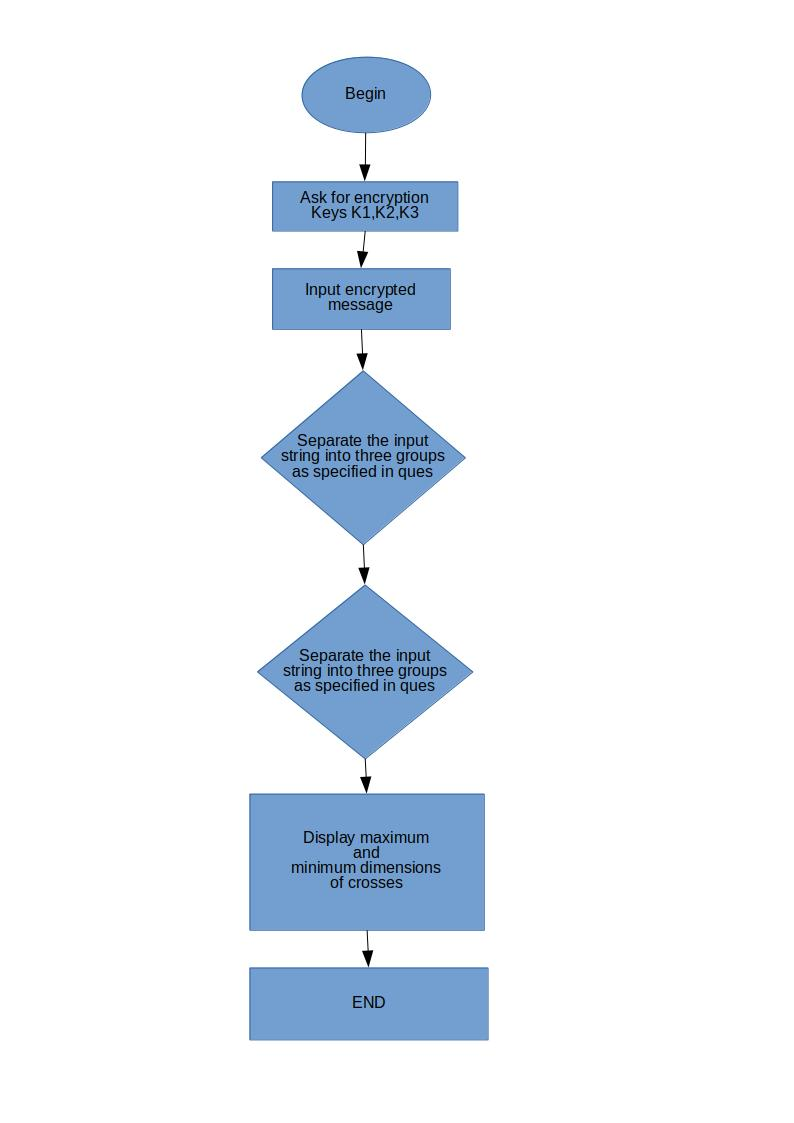
\includegraphics[scale=.5]{ps2flow.jpg}

\subsection{Input Format and output format}
\begin{itemize}
	\item \textbf{Input Format}\\
	Input is key and Encrypted string.
	\item \textbf{Output Format}\\
	Output is Decrypted String
\end{itemize}
	\subsection{Test Cases}
\begin{enumerate}
	\item Input
	1 1 1\\
	bktcluajs\\
	\item Output \\
	ajsbktclu
	
\end{enumerate}

\subsection{Screen-shots}
\begin{figure}
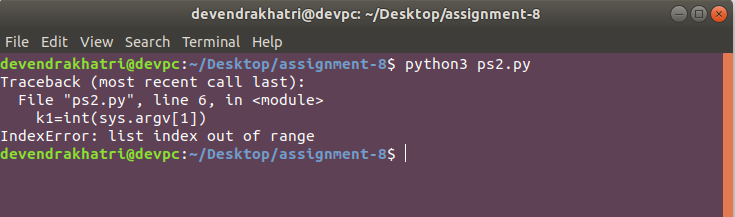
\includegraphics[scale=0.4]{ps2o.png}
\caption{ps2}
\label{fig:fig2}
\end{figure}
\newpage

\section{Appendix}
\subsection{Appendix-A: code for ps1}
\lstinputlisting{ps1.py}


\newpage
\subsection{Appendix-B:code for ps2}
\lstinputlisting{ps2.py}



\newpage
\newpage
\nocite{*}
\bibliographystyle{plain}
\bibliography{bibreport}
\end{document}